\section{Ejercicio Nº 1}
Se desea calcular la distancia recorrida (m) por un móvil que tiene velocidad
constante ($m/s$) durante un tiempo t\@(s) considerar que es un MRU (Movimiento
Rectilíneo Uniforme).
\subsection{Conocimientos Previos}
Fórmula general del MRU\@:
\[D = v\times t\]
\sdconditions[12cm]{azzul}{Donde:}{%
	\begin{tabular}{lcl}
		$D$ & \@: & Distancia \\
		$v$ & \@: & Velocidad \\
		$t$ & \@: & Tiempo
	\end{tabular}
}
\subsection{Solución}
Para la solución a este programa vamos a necesitar que el usuario ingrese la
velocidad y el tiempo, para luego calcular la distancia recorrida, mediante la
fórmula y al final se mostrará en pantalla el valor de la distacia.
\begin{longlisting}
	\sypycode[vs]{python}{linenos,firstnumber=1,firstline=2}{contorCode}{margenCode}{fondoCode}{Files/exercise_i.py}
	\caption{Ejercicio nº 1.}\label{cod:ex_1}
\end{longlisting}
\subsection{Resultados}
\begin{minipage}{14cm}
	\begin{minted}[frame=single,rulecolor=gray,style=perldoc,breaklines,fontsize=\small]{python}
  Ingrese los datos
  Velocidad: 20
  Tiempo: 2
  Distancia: 40 m
	\end{minted}
\end{minipage}
\newpage
% ! --------------------------------------------------------------------------------
\section{Ejercicio Nº 2}
Se necesita obtener el promedio simple de un estudiante a partir de sus tres
notas parciales $N_1$, $N_2$, $N_3$.
\subsection{Conocimientos Previos}
El promedio se obtiene a través de una media aritmética ($\overline{x}$):
\begin{align*}
	\overline{x} & = \cfrac{1}{n}\sum_{i=0}^n {x_i} \\
	             & = \frac{x_1 + x_2 + x_3}{n}
\end{align*}
\subsection{Solución}
En este problema nos pide calcular el promedio a partir de tres notas, para
ello usaremos la fórmula de la media aritmética, sin antes haber solicitado las
notas al usuario finalmente debemos mostrar en pantalla el resultado del
promedio.
\begin{longlisting}
	\sypycode[vs]{python}{linenos,firstnumber=1,firstline=2}{contorCode}{margenCode}{fondoCode}{Files/exercise_2.py}
	\caption{Ejercicio nº 2.}\label{cod:ex_2}
\end{longlisting}
\subsection{Resultados}
\begin{minted}[frame=single,rulecolor=gray,style=perldoc,breaklines,fontsize=\small]{python}
  Calcular Promedio 
  Ingrese las notas:
  Nota 1: 13
  Nota 2: 17
  Nota 3: 16
  Promedio: 15.33
\end{minted}
% ! --------------------------------------------------------------------------------
\section{Ejercicio Nº 3}
Se necesita elaborar un algoritmo que solicite el número de respuestas
correctas, incorrectas y en blanco, correspondientes a postulantes, y muestre
su puntaje final considerando que por cada respuesta correcta tendrá $3$
puntos, respuestas incorrectas tendrá $-1$ y respuestas en blanco tendrá $0$.
\subsection{Solución}
El problema dado nos indica asignar un valor a cada evento, para luego sumarlos
y mostrar el resultado final. Ahora nuestro puntaje final se dará multiplicando
la cantidad de veces por el valor de cada evento. Entonces podriamos omitir el
evento caundo su respuesta es en blanco. En si solo estariamos operando con dos
eventos, el de las respuestas correctas y las incorrectas. \vspace{8mm}
\begin{longlisting}
	\sypycode[vs]{python}{linenos,firstnumber=1,firstline=2}{contorCode}{margenCode}{fondoCode}{Files/exercise_3.py}
	\caption{Ejercicio nº 3.}\label{cod:ex_3}
\end{longlisting}
\subsection{Resultados}
En este ejercicio usaremos como datos: respuestas correctas a 4, respuestas
incorrectas a 10 y respuestas en blanco a 0, entonces el resultado final será:
$4(3) + 10(-1) = 2$.
\begin{minted}[frame=single,rulecolor=gray,style=perldoc,breaklines,fontsize=\small]{python}
  Programa Puntaje Final
  Ingrese los siguientes datos:
  Respuestas correctas: 4
  Respuestas incorrectas: 10
  Respuestas blanco:0
  Puntaje final: 2
\end{minted}
% ! --------------------------------------------------------------------------------
\section{Ejercicio Nº 4}
Elaborar un algoritmo que permita ingresar el número de partidos ganados,
perdidos y empatados, por ABC club en el torneo apertura, se debe de mostrar su
puntaje total, teniendo en cuenta que por cada partido ganado obtendrá 3
puntos, empatado 1 punto y perdido 0 puntos.
\subsection{Solución}
\begin{longlisting}
	\sypycode[vs]{python}{linenos,firstnumber=1,firstline=2}{contorCode}{margenCode}{fondoCode}{Files/exercise_4.py}
	\caption{Ejercicio nº 4.}\label{cod:ex_4}
\end{longlisting}
\subsection{Resultados}
\begin{minted}[frame=single,rulecolor=gray,style=perldoc,breaklines,fontsize=\small]{python}
  Programa Puntaje Total
  Ingresar Datos:   
  Partidos Ganados: 5
  Partidos Perdidos: 10
  Partidos Empatados: 3
  Puntaje Total: 18
\end{minted}
% ! --------------------------------------------------------------------------------
\section{Ejercicio Nº 5}
Elaborar un algoritmo que permita calcular el número de micro discos 3 .5
necesarios para hacer una copia de seguridad, de la información almacenada en
un disco cuya capacidad se conoce. Hay que considerar que el disco duro está
lleno de información, además expresado en gigabyte. Un micro disco tiene 1.44
megabyte y un gigabyte es igual a 1,024 megabyte.
\subsection{Solución}
\begin{longlisting}
	\sypycode[vs]{python}{linenos,firstnumber=1,firstline=2}{contorCode}{margenCode}{fondoCode}{Files/exercise_5.py}
	\caption{Ejercicio nº 5.}\label{cod:ex_5}
\end{longlisting}
\subsection{Resultados}
\begin{minted}[frame=single,rulecolor=gray,style=perldoc,breaklines,fontsize=\small]{python}
  Programa Calcular Número de Micro Discos
  Ingrese tamaño del almacenamiento: 2
  Número de discos necesarios: 1423
\end{minted}
% ! --------------------------------------------------------------------------------
\section{Ejercicio Nº 6}
Se tiene los puntos A y B en el cuadrante positivo del plano cartesiano,
elabore el algoritmo que permita obtener la distancia entre A y B.
\begin{figure}[H]
	\centering
	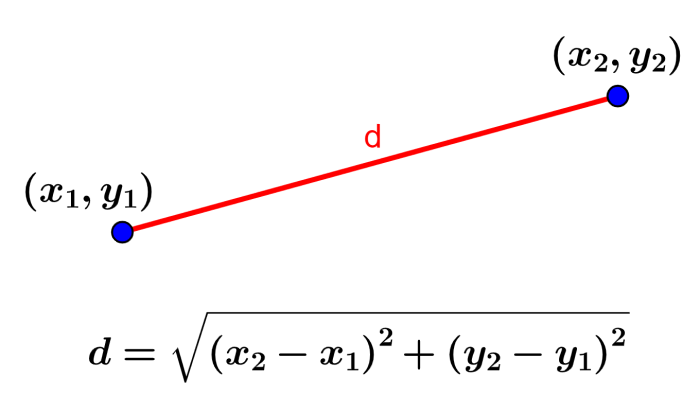
\includegraphics[width=0.5\textwidth]{Images/img1.jpg}
	\caption{Distancia entre A y B}\label{fig:fg1}
\end{figure}
\subsection{Conocimientos Previos}
\subsubsection{Definición Técnica}
La distancia entre dos puntos de dimensión R en el espacio es la aplicación de
la raíz cuadrada al vector que forman esos puntos ordenados. En otras palabras,
la distancia entre dos puntos en el espacio es el módulo del vector formado por
dichos puntos. La distancia entre dos puntos no es nada más que el módulo del
vector que forman los puntos dados. Una vez calculado el módulo del vector, ya
tendremos la distancia entre los dos puntos.
\subsubsection{Fórmula}
Dados los siguientes dos puntos:
\[A(x_1, y_1)\text{ y } B(x_2, y_2)\]
Entonces, la distancia entre estos dos puntos será el módulo del vector que
forman:
\[|\overrightarrow{AB}|=\sqrt{{(x_2-x_1)}^2+{(y_2-y_1)}^2}\]

Será está fórmula con la cual daremos solución a este ejercicio.
\subsection{Solución}
\begin{longlisting}
	\sypycode[vs]{python}{linenos,firstnumber=1,firstline=2}{contorCode}{margenCode}{fondoCode}{Files/exercise_6.py}
	\caption{Ejercicio nº 6.}\label{cod:ex_6}
\end{longlisting}
\subsection{Resultados}
\begin{minted}[frame=single,rulecolor=gray,style=perldoc,breaklines,fontsize=\small]{python}
  Programa Calcular Distancia Entre Dos Puntos
  Ingrese los sigueintes datos
  Para el primer punto:
  Coordenada x: 1
  Coordenada y: 1
  Para el segundo punto:
  Coordenada x: 4
  Coordenada y: 5
  Distancia entre los dos puntos: 5.00
\end{minted}
% ! --------------------------------------------------------------------------------
\section{Ejercicio Nº 7}
Elaborar un algoritmo que solicite 2 números y muestre el promedio de ambos.
\subsection{Conocimientos Previos}
Usaremos misma definición del ejercio Nº 2 (\textbf{Código }\ref{cod:ex_2}).
\subsection{Solución}
\begin{longlisting}
	\caption{Ejercicio nº 7.}\label{cod:ex_7}
	\sypycode[vs]{python}{linenos,firstnumber=1,firstline=2}{contorCode}{margenCode}{fondoCode}{Files/exercise_7.py}
\end{longlisting}
\subsection{Resultados}
\begin{minted}[frame=single,rulecolor=gray,style=perldoc,breaklines,fontsize=\small]{python}
  Programa Calcular Promedio de Dos Números
  Ingrese los números:
  Número 1: 14
  Número 2: 12
  Promedio: 13.00
\end{minted}
% ! --------------------------------------------------------------------------------
\section{Ejercicio Nº 8}
Construya un diagrama de flujo tal que, dado como datos la base y la altura de
un rectángulo, calcule el perímetro y la superficie de este.
\subsection{Conocimientos Previos}
\begin{figure}[H]
	\centering
	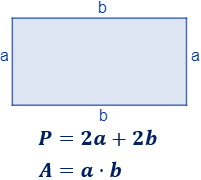
\includegraphics[width=4.5cm]{Images/img2.png}
	\caption{Perímetro y Superficie de un Rectángulo}\label{fig:fg2}
\end{figure}
\sdconditions[12cm]{azzul}{Donde:}{%
	\begin{tabular}{lcl}
		$P$    & \@: & Perímetro            \\
		$A$    & \@: & Área                 \\
		$a, b$ & \@: & Lados del rectángulo
	\end{tabular}
}
\subsection{Solución}
\begin{longlisting}
	\sypycode[vs]{python}{linenos,firstnumber=1,firstline=2}{contorCode}{margenCode}{fondoCode}{Files/exercise_8.py}
	\caption{Ejercicio nº 8.}\label{cod:ex_8}
\end{longlisting}
\subsection{Resultados}
\begin{minted}[frame=single,rulecolor=gray,style=perldoc,breaklines,fontsize=\small]{python}
  Programa Calcular Perímetro y Superficie
  Ingrese los datos:
  [1] Base: 4       
  [2] Altura: 5
  El perímetro es 18.00 y su superficie es 20.00
\end{minted}
% ! --------------------------------------------------------------------------------
\section{Ejercicio Nº 9}
Construya un diagrama de flujo (DF) que resuelva un problema que tiene una
gasolinera. Los dispensadores de esta registran lo que “surten” en galones,
pero el precio de la gasolina está fijado en litros. El DF debe calcular e
imprimir lo que hay que cobrarle al cliente.
\subsection{Diagrama de Flujo de Datos (DFD)}
\begin{figure}[H]
	\centering
	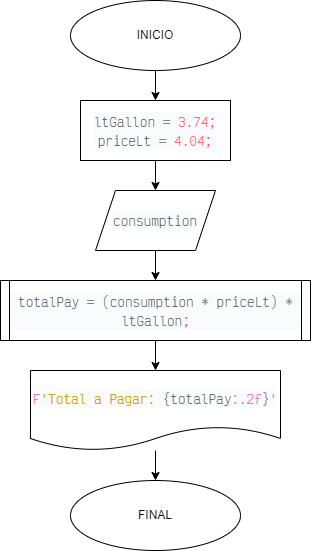
\includegraphics[width=5cm]{Images/ex9.png}
	\caption{Diagrama de Flujo de Datos}\label{fig:fg3}
\end{figure}
\subsection{Solución}
\begin{longlisting}
	\caption{Ejercicio nº 9.}\label{cod:ex_9}
	\sypycode[vs]{python}{linenos,firstnumber=1,firstline=2}{contorCode}{margenCode}{fondoCode}{Files/exercise_9.py}
\end{longlisting}
\subsection{Resultados}
\begin{minted}[frame=single,rulecolor=gray,style=perldoc,breaklines,fontsize=\small]{python}
  Programa Calcular Total a Pagar
  Ingrese candtidad Consumida: 2
  Total a Pagar: 30.22
\end{minted}
% ! --------------------------------------------------------------------------------
\section{Ejercicio Nº 10}
Construya un DF tal que, dado como datos el radio y la altura de un cilindro,
calcule e imprima el área y su volumen.
\subsection{Conocimientos Previos}
\begin{multicols}{2}
	\begin{figure}[H]
		\centering
		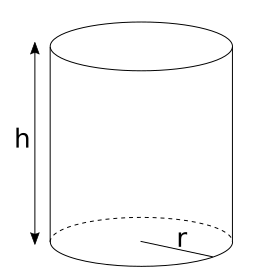
\includegraphics[width=3cm]{Images/img3.png}
		\caption{Ilustración de un Cilindro}\label{fig:fg4}
	\end{figure}
	\[A = 2\times\pi {r}^2\times (r + h)\]
	\[V = \pi\times {r}^2\times h\]
\end{multicols}
\sdconditions[12cm]{azzul}{Donde:}{%
	\begin{tabular}{lcl}
		$A$ & \@: & Área    \\
		$V$ & \@: & Volumen \\
		$r$ & \@: & Radio   \\
		$h$ & \@: & Altura
	\end{tabular}
}
\subsection{Diagrama de Flujo de Datos (DFD)}
\begin{figure}[H]
	\centering
	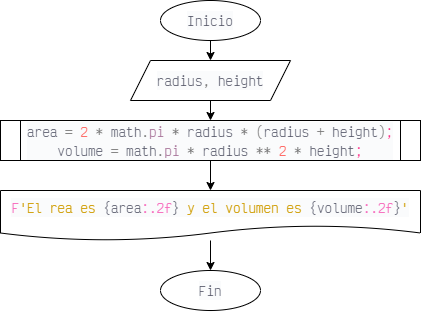
\includegraphics[width=10cm]{Images/ex10.png}
	\caption{Diagrama de Flujo de Datos}\label{fig:fg5}
\end{figure}
\subsection{Solución}
\begin{longlisting}
	\caption{Ejercicio nº 10.}\label{cod:ex_10}
	\sypycode[emacs]{python}{linenos,firstnumber=1,firstline=2}{contorCode}{margenCode}{fondoCode}{Files/exercise_10.py}
\end{longlisting}
\subsection{Resultados}
\begin{minted}[frame=single,rulecolor=gray,style=perldoc,breaklines,fontsize=\small]{python}
  Programa Calcular Área y Volumen del Cilindro
  Ingrese el radio: 3
  Ingrese la altura: 4
  El rea es 131.95 y el volumen es 113.10
\end{minted}